% Chapter 1

\chapter{A sequential implementation for the Odroid-XU developer board}

\lhead{Chapter 5. \emph{A sequential implementation}} % This is for the header on each page - perhaps a shortened title

%----------------------------------------------------------------------------------------
Finally, we turn our attention to define and implement a sequential version of our gesture recognition approach that can run in real-time on an embedded device and which could be suitable for real-world application. To this aim, we modify and improve the classification module of our gesture recognition algorithm, replacing the simple linear SVM classifier with a more complex Structural SVM implementation, designed to take into account time, and choose the Odroid-XU developer board as our target plaform. To make our implementation capable of running in real-time, we exploit several optimization techniques.

We evaluate the Structural SVM implementation by Altun \etal using feature vectors generated from our gesture recognition algorithm. We modify the source code provided by Joachims \cite{joachims} in order to include higher order label-label and label-features interactions, so that the generic 
$\Psi(\mathbf{x},\mathbf{y})$ takes the following form:

\begin{equation}
\Psi_{\epsilon,\tau}(\mathbf{x},\mathbf{y}) = \left( \begin{array}{cc} \sum_{t=1}^T \Phi(\mathbf{x}^t) \otimes  \Lambda^c(y^{t-\epsilon}) \otimes ... \otimes \Lambda^c(y^t) \\ \eta\sum_{t=1}^{T}  \Lambda^c(y^{t-\tau}) \otimes ... \otimes \Lambda^c(y^t) \end{array} \right)
\end{equation}

where $\epsilon$ is the order of label-label dependencies, and $\tau$ is the order of label-features dependencies.

Furthermore, we investigate the use of different loss functions and their impact on recognition rates and confusion matrices. We define a generic loss function that exploits a per-token loss function $\delta(y^t,y'^t)$: $\Delta(\mathbf{y},\mathbf{y'}) = \sum_{t=1}^T \delta(y^t,y'^t)$, and propose two different per-token loss functions:

\begin{equation}
\delta_0(y,y') = \begin{cases} 0 \quad \text{if } y= y'  \\ 
1 \quad \text{otherwise}\end{cases}
\end{equation}

\begin{equation}
\delta_1(y,y') = \begin{cases} 0 \quad \text{if } y= y'  \\ 
3 \quad \text{if } y=8, y' \neq 8 \lor y\neq8, y'=8  \\
1 \quad \text{otherwise}\end{cases}
\end{equation}

\section{The Odroid-XU board}
Our cultural heritage system consists of a collection of wearable ego-vision devices, that embed a glass-mounted camera and an Odroid-XU developer board, serving as video-processing and network communication unit.
There are several benefits in using such a portable device: the commercial availability and low costs for prototypes evaluation, the computational power and energy efficiency of the Big-Little architecture. Furthermore it has the possibility  of peripheral addition to extend connections and input devices. 

\begin{figure}[t!]
\centering
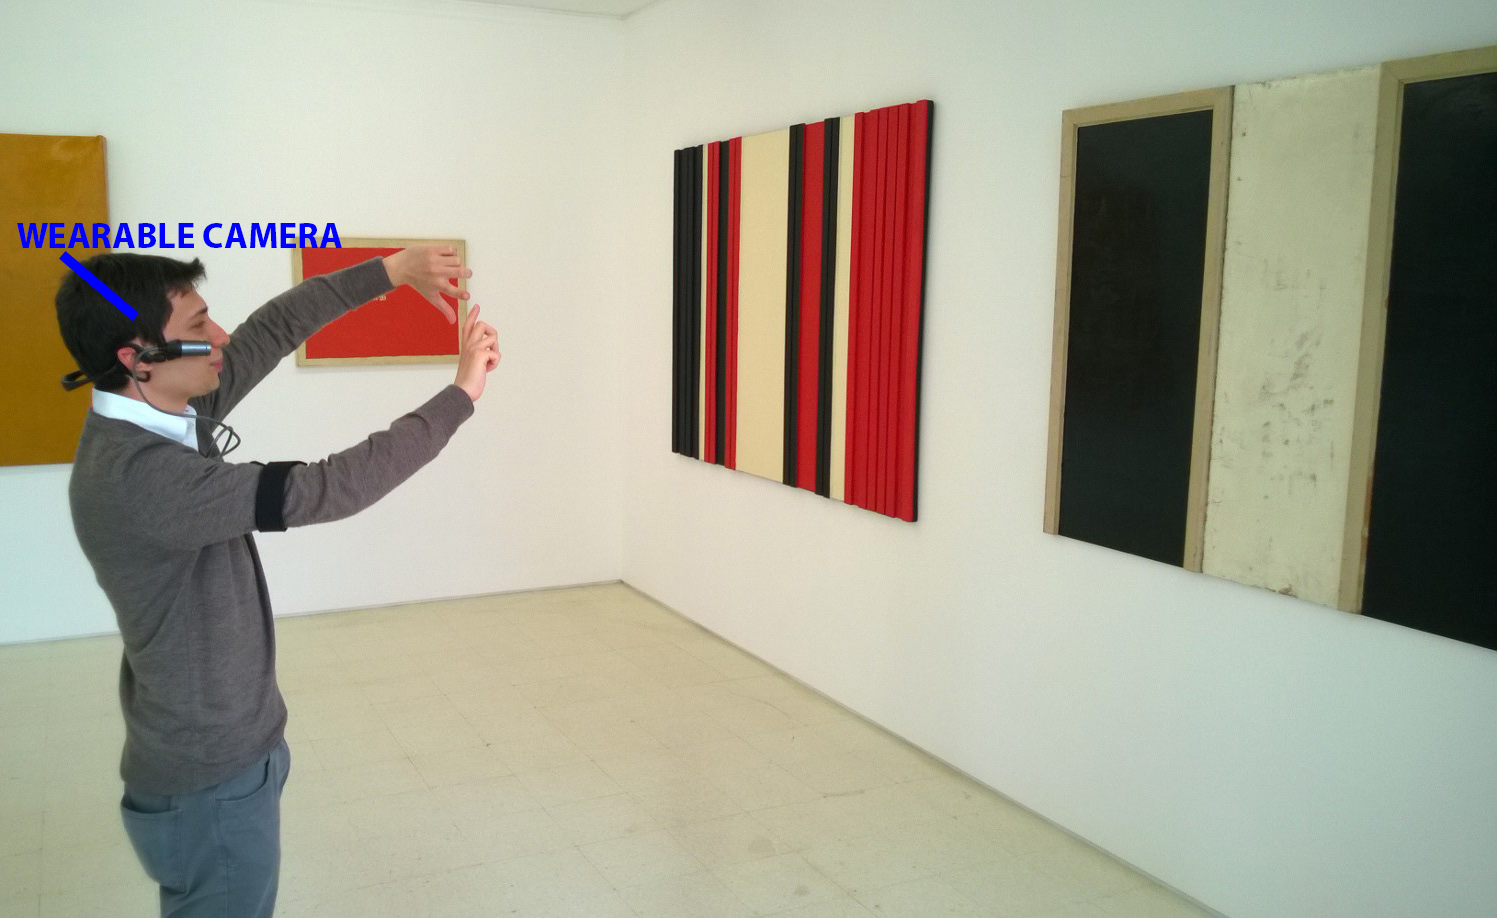
\includegraphics[width=0.5\linewidth]{Figures/lore_maramotti.jpg}
\caption{User interacting with wearable camera.}
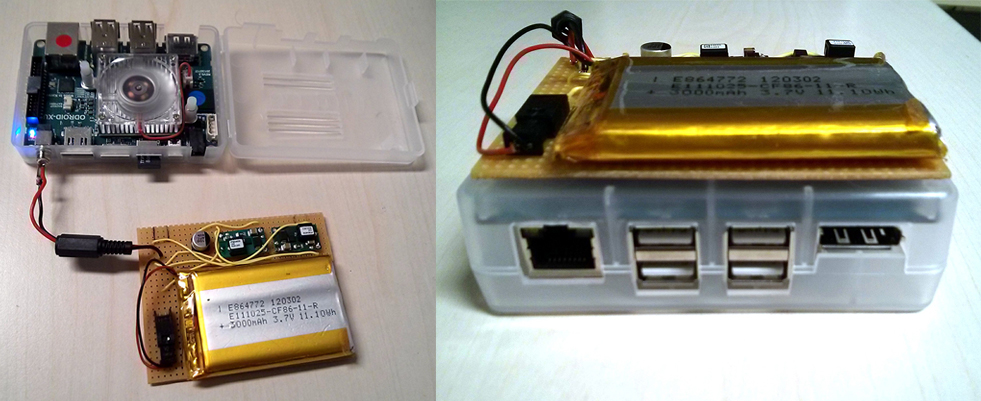
\includegraphics[width=0.5\linewidth]{Figures/board.jpg}

\caption{The Odroid-XU board with battery pack.}
\label{board}
\end{figure}

Hardkernel have made a name for themselves within the open-source community by delivering high performance development boards at affordable prices. The Odroid-XU platform boasts an Exynos 5 Octa processor – the same SoC found inside the Samsung Galaxy S4, which includes a PowerVR SGX544MP3 GPU clocked at around 600 MHz (see figure \ref{odroid-xu}).

The key features and specifications of the ODROID-XU development board include:
\begin{itemize}
\item big.LITTLE processing based on the Cortex™-A15 and Cortex™-A7 quad core CPUs
\item PowerVR SGX544MP3 GPU (OpenGL ES 2.0, OpenGL ES 1.1, OpenCL 1.1 EP, Renderscript/Filterscript)
\item 2Gbyte LPDDR3 PoP (1600Mbps/pin, 2 x 32bit Bus)
\item USB 3.0 Host x 1, OTG x 1, USB 2.0 Host x 4
\item HDMI 1.4a output Type-D connector (Micro-HDMI)
\item eMMC 4.5 Flash Storage
\item Micro-SD socket
\item MIPI DSI for LCD display output
\item On-board Audio Codec
\item Fast 10/100 Ethernet LAN
\item WiFi
\item 5V/4A power supply
\end{itemize}

Big.LITTLE is a heterogeneous computing architecture developed by ARM that couples slower, low-power processor cores with more powerful and power-hungry ones. The intention being to create a multi-core processor that can adjust better to dynamic computing needs and use less power than clock scaling alone. In this case we have the Cortex-A7 coupled with the Cortex-A15, which have been designed to be architecturally compatible.

In the Samsung Exynos 5 there is only one way for the different processor cores to be arranged in a big.LITTLE design: the \textit{clustered model} approach. With this approach the operating system scheduler can only see one of the two processor clusters, when the load on one cluster hits a certain point, the system transitions to the other cluster. All relevant data is passed through the common L2 cache, the first core cluster is powered off and the other one is activated. A Cache Coherent Interconnect (CCI) is used.




\begin{figure}[t!]
\centering
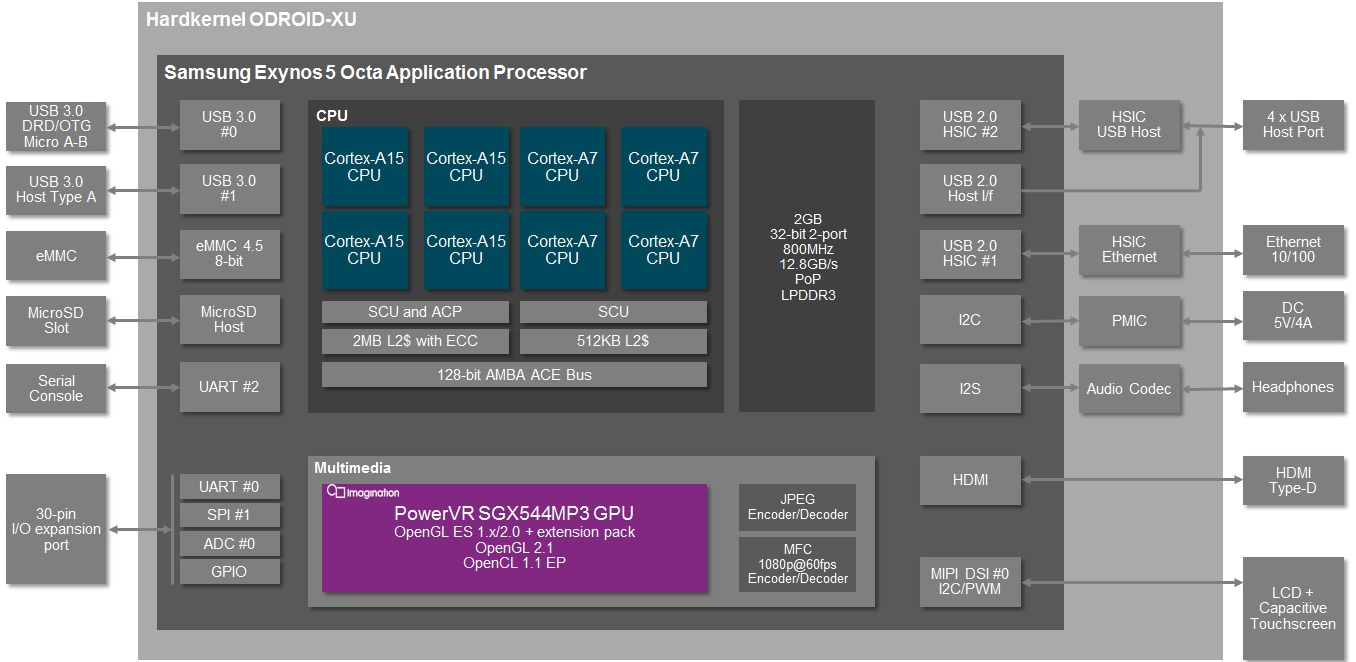
\includegraphics[width=0.9\linewidth]{Figures/Hardkernel-ODROID-XU-block_diagram.jpg}
\caption{Hardkernel Odroid-XU block diagram}
\label{odroid-xu}
\end{figure}

\section{Implementation}
\lstset{language=C++}

As stated before, on the Odroid-XU board only one of the two clusters can run at the same time. Since our application is heavy, we choose the A15 cluster, which includes four cores and is the most performant cluster. This is done trough the following command:
\begin{lstlisting}[frame=single]  % Start your code-block

echo performance > /sys/devices/system/cpu/cpu0/cpufreq/scaling_governor
\end{lstlisting}
which basically activates the \verb+performance+ governor as the controller for the big.LITTLE switching mechanism.
Then, having written a sequential implementation of our algorithm using the OpenCV library\footnote{This is joint work with Francesco Paci.}, we compile it using \verb+gcc+ with the following options:
\begin{lstlisting}[frame=single]  % Start your code-block

-g -mfpu=neon-vfpv4 -ftree-vectorize -mfloat-abi=hard -mtune=cortex-a15 -marm
\end{lstlisting}

The \verb+-g+ flag tells the compiler to produce debugging information in the operating system's native format, \verb+-mfpu=neon+  specifies what floating-point hardware (or hardware emulation) is available on the target, \verb+-ftree-vectorize+ enables the auto-vectorizer (which will try to use SIMD instructions, when possible), \verb+-mfloat-abi=hard+ allows generation of floating-point instructions and uses FPU-specific calling conventions, and \verb+-mtune=cortex-a15+ tunes the performance of the compiler for the A15 target.

\subsection{OpenMP and Neon Intrisics}
This first sequential version runs at 4.3 frames/s on $160\times 120$ frames, and needs 234 ms to elaborate each frame. The main bottleneck of this implementation is the multi-scale Farneback's optical flow, which requires 141 ms for each frame to run. Farneback's algorithm is executed two times for each frame, since the optical flow is calculated both on the original frame on the warped one, so we use OpenMP to run these two executions simultaneously on two different threads. Then, we use Neon intrinsics in order to exploit the SIMD capabilities of our CPU and thus gain a better performance on each thread.

A complete explanation of the optimizations made is beyond the purpose of this chapter, but, as an example, let's consider this for loop, which is responsible of 51 of the 234 ms:
\begin{lstlisting}[frame=single]  % Start your code-block

for( ; x < width*5; x++ ) {
	float s0 = srow[m][x]*kernel[0];
	for( i = 1; i <= m; i++ )
		s0 += (srow[m+i][x] + srow[m-i][x])*kernel[i];
	vsum[x] = s0;
}
\end{lstlisting}

Once optimized with Neon SIMD, the previous code becomes:
\begin{lstlisting}[frame=single]  % Start your code-block

int xstart = x;
float kernelext0[4];
fill_n(kernelext0,4,kernel[0]);
for( ; x < width*5-4; x+=4 ) {
           vst1q_f32(vsum+x, vmulq_f32(vld1q_f32(srow[m]+x),
		vld1q_f32(kernelext0)));
}
float a[width*5];
float kernelext[4];
for( i = 1; i <= m; i++ ) {
	fill_n(kernelext, 4, kernel[i]);
           for (x=xstart; x<width*5-4; x+=4) {
                        vst1q_f32(a+x, vaddq_f32(vld1q_f32(srow[m+i]+x), 
			vld1q_f32(srow[m-i]+x)));
                        vst1q_f32(vsum+x, vmlaq_f32(vld1q_f32(vsum+x), 
			vld1q_f32(a+x), vld1q_f32(kernelext)));
           }
}
\end{lstlisting}
As can be seen, the two for loops have been inverted and four floats are processed at each iteration. The new code block takes only 20 ms to run. 

\subsection{Further optimizations}
Having included several OpenMP/SIMD optimizations, our code runs at 7.1 frames/s on the A15 cluster, still not enough for real-time. Moreover, our algorithm needs an high frame rate in order to compute significant trajectories. Being the Farneback's algorithm our main bottleneck, we could turn our attention to the PowerVR GPU embedded into the Odroid board. Unfortunately, Hardkernel has not yet released an Ubuntu kernel that supports the PowerVR GPU\footnote{see: \url{http://forum.odroid.com/viewtopic.php?f=61&t=2236}.}, so the only way we have to increase speed is to further reduce the frame size and keep only one level of the spatial pyramid. Having reduce the frame size to $113\times 85$


... the Farneback's optical flow\footnote{\url{https://github.com/Itseez/opencv/blob/9aa4410509fcc60dfabb78c14a96ed5153ee117e/modules/ocl/src/opencl/optical_flow_farneback.cl}} is included in the C++ code.


\section{Some applications}
\subsection{Ego-Vision Jacket}
\subsection{...}
